\chapter{Results}
\label{result}

Semantic Knowledge Management Framework was developed with a focus on six quality goals. These goals are reliability, scalability, testability, maintainability, usability, and security. Progress was made, to some degree, in meeting each of the quality goals. Some of the goals, however, could not be thoroughly evaluated due to missing functionality or unavailable resources. None of them can be considered fully met in the current state of SKMF. What follows is a discussion of the different quality goals, the motivation behind them, the level of success in meeting them, and what is still required to properly fulfill them. The first three goals and their outcomes are discussed in the first section of this chapter. Each of the three remaining goals is discussed in a separate section.


\section{Unverified Quality Goals}
\label{result:unverified}

Any system that is part of vital business operations should be reliable and SKMF could find itself in that position. Reliability also supports availability, which is a tenet of good security. To support this goal, exceptions in SKMF are caught and reported without re-raising only at areas where program operation is not compromised by failure of the current operation. Also, consistency checks are made whenever an operation would alter data in the triplestore. There is, however, much still to do to ensure reliability. For one, extensive negative testing is required to ensure sane handling of unexpected inputs. Tests must also be performed in a multi-client setting to ensure that competing requests to not cause reliability issues. Only when SKMF can perform under duress for extended periods of time can this goal be considered achieved.

Scalability is another goal that is directed toward business environments. In order to scale to large, multisystem environments, SKMF utilizes a multi-threaded framework for handling Web content. It also separates itself from the Web server process and SPARQL endpoint so that these components may be implemented using something that suits the needs of the organization. Unfortunately, there are some serious shortcomings in the prototype implementation of SKMF. While the Web framework uses multi-threading, SKMF does not make use of threads for backend operations. A bigger issue with scaling comes from a lack of caching, which results in excessive queries to the SPARQL endpoint. This problem would be particularly detrimental in a multi-user environment with frequent system accesses. A final improvement to support scalability is to offload some tasks, most notably password hashing, onto the client. Again, failure to do this would have greater consequences in a multi-user environment. Once these measures are taken, satisfactory scalability could be considered achieved once SKMF is capable of processing requests on par with the Web server behind which it operates.

Since SKMF initially followed test-driven development, the goal of testability naturally fit the project. As the project moved away from TDD, however, this goal increasingly waned. The result is a split between testable code and poorly tested code. Test cases exist for all of the model components of SKMF. While not exhaustive, they demonstrate how easily test cases for those components can be written. The view and controller components, on the other hand, have only minimal test cases. The code in these components is also of considerably lower quality than that written for the model, so it is likely more difficult to test. Therefore, to achieve testability, the view and controller code should be cleaned up to better match the model code and proper Flask testing should be used on those components.


\section{Maintainability}
\label{result:maintain}

Maintainability is a personal goal for SKMF. The project may be shelved for some time, then picked up again at some point in the future. It may also be shared or even open-sourced, giving new developers the opportunity to build upon it. In either case, the code should be accessible and understandable to future developers. The interface needs to be clear enough others to use without touching the code, as well. Also, developers should not have to worry about breaking the code in unexpected ways when making modifications. Several steps were taken to ensure the various facets of this goal.

Simplicity promotes maintainability. Whenever possible, Python built-in data structures provide the underlying functionality. This minimizes custom logic and provides developers with familiar constructs. Complex layouts of the data structures follow similar patterns wherever they appear, providing consistency. Documentation accompanies every module, every class, and the vast majority of functions, methods, and attributes. SKMF lacks direct support for internationalization, but consideration of this issue resulted in the migration of most textual output into an English localization file, providing for simpler implementation of i18n at a future time. Templates contain HTML comments to mark their points of entry and exit, which aids in tracking the origin of content in Web views. SKMF avoids the use of deprecated classes and methods, with great care taken to ensure the absence of deprecation warnings from testing branches, where applicable. Finally, SKMF avoids long import chains to minimize coupling. With all of these practices in place, SKMF achieves its highest level of quality in maintainability.

There is still room for improvement. Better separation of concerns between the model and the controller would present more intuitive interfaces. View code requires pruning, modularization, and simplification. There is also an open question of whether to keep the innermost dictionary for SKMF triples modeled after the JSON response for SPARQL queries, keeping those structures directly compatible; or to model them after the outer dictionaries, which would allow all levels of the triples to be handled in a uniform manner, even recursively, if so desired. Naming conventions, while mostly consistent, could use some disambiguation. More improvements may be recognized as more eyes review the code.


\section{Usability}
\label{result:usability}

For a project designed to simplify the user experience when handling semantic data, usability is extremely important. While knowledge management systems, in general, support collection and retrieval of knowledge, SKMF seeks to present users with an intuitive method of interacting with the links that represent such knowledge. Essentially, users should be able to add information to the system with enough detail to easily identify and describe it, create meaningful connections between the new information and the information that already exists in the system, and easily derive meaning from the connections and relationships identified through intuitive queries. Such meaningful user interaction creates the core value for a semantic knowledge management system.

SKMF makes several assumptions on behalf of the user. For one, users tend to prefer simple, natural language labels to complex URIs. Queries, therefore, automatically append optional clauses for these labels, which appear in the user interface wherever the requested resource displays. Also, when new information is added, users are required to provide some, preferably meaningful, descriptions before submitting the form. Another assumption is that users want links to information sources. So, when a textual label for a resource is rendered, it renders as a hyperlink to a page that fully describes that resource, in case the query that retrieved that resource did not retrieve all of the desired connections thereto. An example of the resulting Web page is shown in Figure
\ref{info-page}.
Users are assumed, as well, to be unfamiliar with RDF. To aid these users, SKMF populates dropdown lists with elements categorized by where they are most likely to appear in a triple, with classes separated from properties. An example is shown in Figure
\ref{resource-page}.

\begin{figure}[!ht]
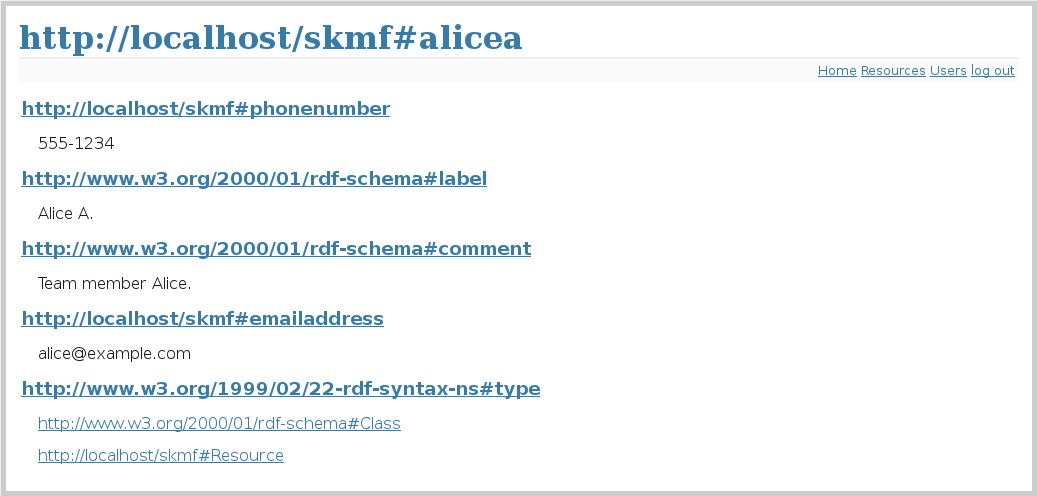
\includegraphics[width=6.5in]{info-page}
\caption[Resource information page of SKMF]
 {\narrower All information about Alice A. in SKMF.
 }
\label{info-page}
\end{figure}

\begin{figure}[!ht]
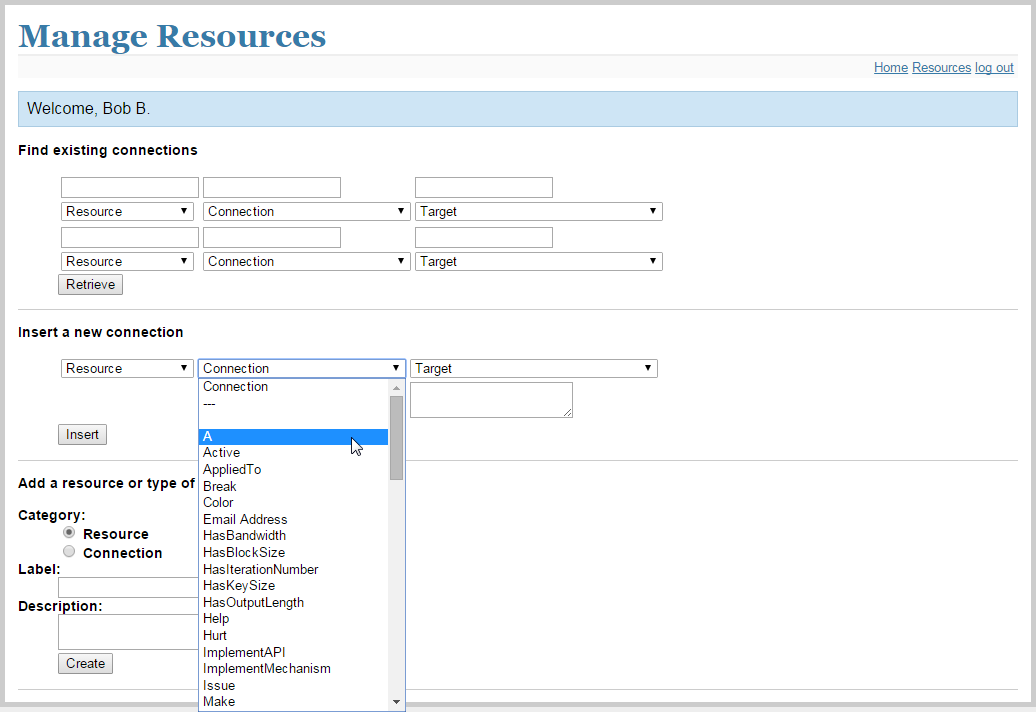
\includegraphics[width=6.5in]{resource-page}
\caption[Resource management page of SKMF]
 {\narrower Web page for managing resources in SKMF. The top form allows for a SPARQL query to be constructed with two sets of constraints. Text fields allow input of variables and dropdowns allow for selection of existing URIs, represented by their labels. The middle form allows for descriptions to be added to an existing resource. The bottom form allows for the addition of a new resource, with the `Label' and `Description' fields both required. A non-default selection from a dropdown always overrides the contents of a text field.
 }
\label{resource-page}
\end{figure}

Unsurprisingly, the usability goals proved overly ambitious for the scope of this project, so the prototype falls short on numerous points. The type of meaningful user interaction desired for SKMF requires implementation of dynamic Web pages with forms that grow in size to support arbitrary levels of refinement. There was insufficient time during this project for the necessary techniques to be learned and implemented. While the code is thoroughly documented, the UI lacks helpful documentation. In addition, a mock case study, discussed in the next section, revealed that some of the assumptions, as they are currently handled, hinder the user experience. For instance, the treatment of resources added to the system becomes awkward when that resource is a person, as many of the attributes one normally associates with people are not immediately available in the forms. Also, the controller automatically appends a language tag to string literals as they are added to help support future internationalization, as discussed in section
\ref{result:maintain}
on maintainability. This places a needless language restriction on numeric strings, such as phone numbers. As the user interface is refined, the basic assumptions require refinement, as well, driven by feedback from potential users.

Aside from a dynamic overhaul of the UI, usability in SKMF would benefit from various backend improvements. Just as textual labels are requested for resources, full descriptions could be requested, as well, and made available to the frontend to use, for instance, in tooltips. Form text could be parsed to determine its purpose, which would allow savvy users to craft more complex queries than the system allows through selections. Subtle exposure of SPARQL functions and their use in the controller would also allow for richer user interaction. A seed ontology would aid the system in performing such actions intelligently. User experience is one area of software development wherein improvements can always be made and SKMF has a lot of potential for growth and experimentation in this area.


\subsection{Mock Case Study}
\label{result:case-study}

In lieu of a full case study, SKMF was partially validated through a mock case study involving only the developer. For that exercise, the STAC
\cite{ontosec}
was imported into SKMF. Outside of SKMF, a short list was made of physical servers, software, team members, known vulnerabilities, and mitigations. In addition, a set of tasks were defined, such as locating servers that were susceptible to certain vulnerabilities and retrieving the contact information of the person responsible for maintaining them. The developer then used SKMF to enter the information from the list and create connections, such as who was responsible for which servers and which vulnerabilities applied to which software packages. Finally, the developer attempted to execute the tasks with a minimal number of steps.

Although it lacked the insight that would have been gained from exposure to outside parties, the mock case study did reveal many of the usability issued found with SKMF. For one, the STAC ontology was not immediately recognized by SKMF because of its reliance on OWL, so support had to be added in code instead of through the user interface. Also, team members could not be assigned names, as are users when they are added to the system, because only the administrative user management interface has access to the `foaf' namespace where many person-centric properties are readily available. The need for proper prompts and help text was also made apparent, as the queries used to fulfill the tasks mostly relied on knowledge SPARQL syntax and likely would not have been constructed properly through the forms by a user who is unfamiliar with SPARQL.

Aside from the shortcoming, the mock case study did validate some of the potential uses for SKMF. Adding resources and applying properties proved to be straightforward. Also, obtaining enough information from a query to follow a link for more information was simple enough to make browsing a viable way to locate information in small datasets. Most importantly, it was demonstrated that queries can return the sort of indirect relationship that SKMF is meant to provide. For instance, one task was to retrieve the phone numbers of the people responsible for any servers affected by a specific vulnerability. By supplying the vulnerability, some specific relationships, and a couple of variables, it was possible to bring up a list of the responsible parties which contained links to their full information, including phone numbers. While this task took two steps in the SKMF prototype interface, it could realistically be reduced to a single step with a more dynamic interface that provides useful prompts to the user.


\section{Security}
\label{result:security}

Since SKMF was developed under the Cyber Security Engineering program at the University of Washington, Bothell, security is an obvious quality goal for the project. Security also serves a practical purpose for an application that is accessible over a network and used to manage sensitive information. Such an application must provide confidentiality, integrity, and availability by enforcing authentication, authorization, and non-repudiation
\cite{incidentresponse}.
Whether an action performed against the system is malicious or unintentionally detrimental, it should not result in violation of the aforementioned tenets within the system, requiring the system to handle these actions in a secure manner. The following sections discuss what threats face a system like SKMF, what safeguards are currently implemented in SKMF to mitigate those threats, and what safeguards should be implemented to provide better mitigation.


\subsection{Ensuring Confidentiality}
\label{result:confidentiality}

A breach of confidentiality in SKMF primarily means disclosure of information from the triplestore to an unauthorized party, as this is the sole repository for information. Interception of a user's credentials is a breach of confidentiality that could lead to spoofing and a larger breach. Such attacks could be made between SKMF and the SPARQL endpoint, between SKMF and the Web server process, or between the Web server and the user. Spoofing attacks are particularly potent because they permit an attacker to bypass most safeguards with little effort.

Data passing between SKMF and the Web server is managed primarily by Flask. So long as Flask communicates with the Web server in a sane manner, transactions should occur sanely, as well. Therefore, SKMF comes with a strong recommendation to deploy it on the same host as the Web server to minimize the opportunity for eavesdropping. It is also recommended that the Web server be configured with TLS, as this is beyond the control of SKMF. Similarly, since SKMF uses pure SPARQL to communicate with the widest possible range of SPARQL endpoints, security between the two is largely a matter of deployment. The triplestore should not be deployed on the same host as the Web server, as this increases the attack surface on a key data asset. Even on an intranet, the triplestore is best deployed on a separate host from SKMF, as SKMF communicates directly with the Web server and may introduce vulnerabilities to the triplestore. SPARQLWrapper, which SKMF uses to connect with the SPARQL endpoint, supports TLS, so it is recommended to pair the triplestore with a SPARQL endpoint that supports TLS. If this is not an option, then a secure tunneling protocol, such as IPsec, should protect the connection.

Flask-Login provides the authentication resources used to govern access to the system. In addition, SKMF counters spoofing by supporting graph-based access controls. Sensitive data may reside in a named graph that is inaccessible to unprivileged users. An example of this is the `user' graph, which is only accessible to the administrative user. By segregating data into graphs, administrators minimize the impact of compromised user credentials. As with any networked system, the administrative credentials are highly sensitive and should be properly safeguarded. The full support for graph-based access control is not exposed in the Web interface, so this needs to be implemented before this feature can adequately protect a deployment.


\subsection{Ensuring Integrity}
\label{result:integrity}

The biggest integrity concern in SKMF is the state of the triplestore. The information retrieved therefrom should accurately reflect the information written thereto. Information in transit also requires integrity, particularly if it results in modification of the triplestore. Loss of integrity may result from malicious tampering or from failure to validate information passed between processes. The latter is easier to protect against within SKMF, as it likely produces detectable defects in the data. Tamper protection requires proactive mitigation.

Many of the safeguards that ensure confidentiality also provide integrity checks. TLS and IPsec both use cryptographic message authentication codes to verify that data were not altered in transit. Most triplestores automatically verify data integrity to prevent corruption. While SKMF does not implement tamper protection, it does provide checks to deter unintended alteration of information. Whenever the user creates a new resource, the triplestore is checked for the existence of a resource that already meets the provided description and, if found, loads that resource instead of creating it anew, alerting the user to the existence of the resource, as well. When updates are performed on a resource, they are first checked against the existing information about that resource to avoid collisions. The sane portions of the update are then applied and their description returned to the user, allowing the user to take appropriate action if the returned description differs from the desired update.

One way to greatly improve checks for inadvertent modification in SKMF would be to provide a description of the changes back to the user and request confirmation before committing them. This may pose a usability issue, though, so it may work best to allow the users to set an option that enables or disables this feature, with an administrative option to override any user's selection. Integrity maintenance could also be improved by coding strict checks for adherence to the RDF and SPARQL specifications into the controller of SKMF to make intelligent decisions about how to treat all data that are destined for the SPARQL endpoint.


\subsection{Ensuring Availability}
\label{result:availability}

If SKMF is not available to legitimate users, then it only serves to consume resources that are better allocated elsewhere. While many aspects of availability depend upon the deployment environment, there are others for which SKMF holds sole responsibility. A process crash would render the system inaccessible until the process could be restarted. Excessive query requests could result in unacceptably slow response times and traffic congestion. It is even possible to cause SKMF to consume excessive processing power by flooding it with login attempts for a legitimate user with the wrong password, since the hashing operation to verify the password is performed on the server. There are other ways to reduce available, but this sampling represent the biggest threats to SKMF.

The prototype of SKMF lacks robust availability assurance. It catches known exceptions during procedures that are not crucial to continuing operation, but there are still procedures that can cause a crash, which an attacker may be able to exploit. Improved error handling would greatly mitigate this vulnerability. Excessive queries currently pose a real threat. As briefly mentioned in section
\ref{result:unverified}
concerning scalability, queries are not cached and performance suffers even with small datasets. A more intelligent query system and a caching mechanism would mitigate attacks involving query floods while providing increased performance to the user. Another issue mentioned with scalability is performing password hashing on the server. The Bcrypt algorithm is used for hashing because it is designed to be slow and requires significant resources to reproduce a hash. To prevent an attacker from abusing this to consume excessing processing power, the hashing operating could be delegated to the client. This would have the added benefit of preventing plain text passwords from crossing the network, reducing the opportunity for interception of credentials and spoofing of users.
